\chapter{Edeka Supermarket Layout and Design / Edeka-Supermarkt-Layout und -Design / 艾德卡超市布局与设计}

\section{Store Layout Overview / Überblick über das Filiallayout / 门店布局概述}

\begin{otherlanguage}{ngerman}
Edeka-Supermärkte folgen einem durchdachten Layout-Konzept, das darauf ausgelegt ist, die Kunden durch den gesamten Laden zu führen und gleichzeitig eine optimale Produktpräsentation zu gewährleisten. Das Layout variiert je nach Filialgröße und Standort, folgt aber grundsätzlichen Prinzipien.
\end{otherlanguage}

Edeka supermarkets follow a thoughtful layout concept designed to guide customers through the entire store while ensuring optimal product presentation. The layout varies by store size and location but follows fundamental principles.

艾德卡超市遵循经过深思熟虑的布局概念，旨在引导顾客走遍整个商店，同时确保最佳的产品展示。布局因门店规模和位置而异，但遵循基本原则。

% Store Floor Plan
\begin{figure}[h]
\centering
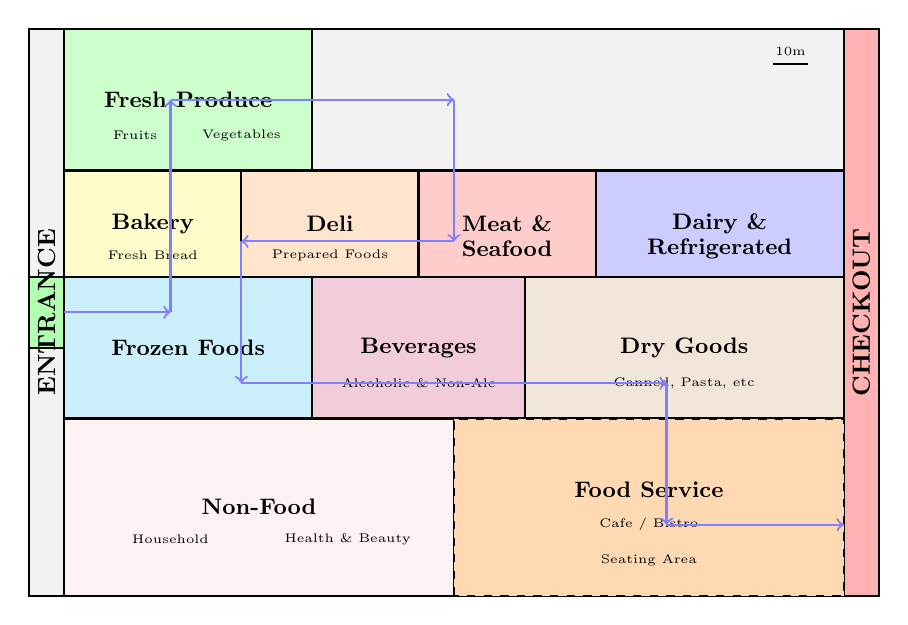
\begin{tikzpicture}[scale=0.9, transform shape]
    % Store outline
    \draw[thick, fill=gray!10] (0,0) rectangle (12,8);
    
    % Entrance
    \draw[thick, fill=green!30] (0,3.5) rectangle (0.5,4.5);
    \node[rotate=90] at (0.25,4) {\textbf{ENTRANCE}};
    
    % Exit/Checkout area
    \draw[thick, fill=red!30] (11.5,0) rectangle (12,8);
    \node[rotate=90] at (11.75,4) {\textbf{CHECKOUT}};
    
    % Fresh produce section (right side, draws customers in)
    \draw[thick, fill=green!20] (0.5,6) rectangle (4,8);
    \node[rotate=0, font=\small\bfseries] at (2.25,7) {Fresh Produce};
    \node[rotate=0, font=\tiny] at (1.5,6.5) {Fruits};
    \node[rotate=0, font=\tiny] at (3,6.5) {Vegetables};
    
    % Bakery section
    \draw[thick, fill=yellow!20] (0.5,4.5) rectangle (3,6);
    \node[rotate=0, font=\small\bfseries] at (1.75,5.25) {Bakery};
    \node[rotate=0, font=\tiny] at (1.75,4.8) {Fresh Bread};
    
    % Deli and prepared foods
    \draw[thick, fill=orange!20] (3,4.5) rectangle (5.5,6);
    \node[rotate=0, font=\small\bfseries] at (4.25,5.25) {Deli};
    \node[rotate=0, font=\tiny] at (4.25,4.8) {Prepared Foods};
    
    % Meat and seafood
    \draw[thick, fill=red!20] (5.5,4.5) rectangle (8,6);
    \node[rotate=0, font=\small\bfseries] at (6.75,5.25) {Meat \&};
    \node[rotate=0, font=\small\bfseries] at (6.75,4.9) {Seafood};
    
    % Dairy and refrigerated
    \draw[thick, fill=blue!20] (8,4.5) rectangle (11.5,6);
    \node[rotate=0, font=\small\bfseries] at (9.75,5.25) {Dairy \&};
    \node[rotate=0, font=\small\bfseries] at (9.75,4.9) {Refrigerated};
    
    % Frozen foods (back wall)
    \draw[thick, fill=cyan!20] (0.5,2.5) rectangle (4,4.5);
    \node[rotate=0, font=\small\bfseries] at (2.25,3.5) {Frozen Foods};
    
    % Beverages
    \draw[thick, fill=purple!20] (4,2.5) rectangle (7,4.5);
    \node[rotate=0, font=\small\bfseries] at (5.5,3.5) {Beverages};
    \node[rotate=0, font=\tiny] at (5.5,3) {Alcoholic \& Non-Alc};
    
    % Dry goods and pantry
    \draw[thick, fill=brown!20] (7,2.5) rectangle (11.5,4.5);
    \node[rotate=0, font=\small\bfseries] at (9.25,3.5) {Dry Goods};
    \node[rotate=0, font=\tiny] at (9.25,3) {Canned, Pasta, etc};
    
    % Non-food section
    \draw[thick, fill=pink!20] (0.5,0) rectangle (6,2.5);
    \node[rotate=0, font=\small\bfseries] at (3.25,1.25) {Non-Food};
    \node[rotate=0, font=\tiny] at (2,0.8) {Household};
    \node[rotate=0, font=\tiny] at (4.5,0.8) {Health \& Beauty};
    
    % Food service area (cafe/bistro)
    \draw[thick, fill=orange!30, dashed] (6,0) rectangle (11.5,2.5);
    \node[rotate=0, font=\small\bfseries] at (8.75,1.5) {Food Service};
    \node[rotate=0, font=\tiny] at (8.75,1) {Cafe / Bistro};
    \node[rotate=0, font=\tiny] at (8.75,0.5) {Seating Area};
    
    % Customer flow arrows
    \draw[->, thick, blue!50] (0.5,4) -- (2,4);
    \draw[->, thick, blue!50] (2,4) -- (2,7);
    \draw[->, thick, blue!50] (2,7) -- (6,7);
    \draw[->, thick, blue!50] (6,7) -- (6,5);
    \draw[->, thick, blue!50] (6,5) -- (3,5);
    \draw[->, thick, blue!50] (3,5) -- (3,3);
    \draw[->, thick, blue!50] (3,3) -- (9,3);
    \draw[->, thick, blue!50] (9,3) -- (9,1);
    \draw[->, thick, blue!50] (9,1) -- (11.5,1);
    
    % Scale indicator
    \draw[thick] (10.5,7.5) -- (11,7.5);
    \node[above, font=\tiny] at (10.75,7.5) {10m};
\end{tikzpicture}
\caption{Typical Edeka Supermarket Floor Plan / Typisches Edeka-Supermarkt-Layout / 典型艾德卡超市平面图}
\end{figure}

\section{Section-by-Section Breakdown / Detaillierte Sektionsaufteilung / 各区域详细分解}

\subsection{Fresh Produce Section / Frischwarenabteilung / 生鲜区}

\begin{otherlanguage}{ngerman}
Die Frischwarenabteilung befindet sich typischerweise direkt beim Eingang, um Kunden sofort mit frischen, ansprechenden Produkten zu begrüßen. Dies ist eine bewährte Strategie im Einzelhandel.
\end{otherlanguage}

The fresh produce section is typically located directly at the entrance to immediately greet customers with fresh, appealing products. This is a proven retail strategy.

生鲜区通常位于入口处，以便立即用新鲜、吸引人的产品迎接顾客。这是经过验证的零售策略。

% Produce Section Detail
\begin{figure}[h]
\centering
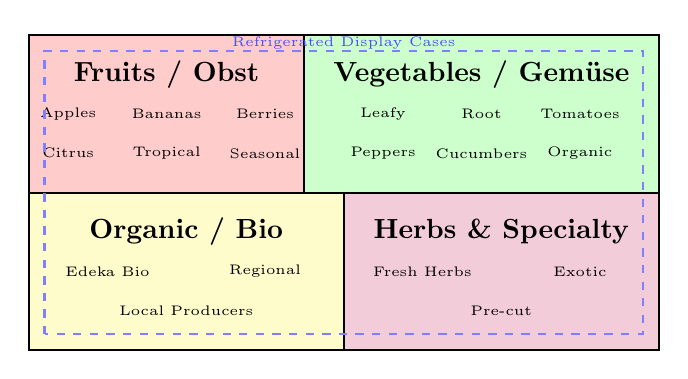
\begin{tikzpicture}[scale=1.0]
    % Section outline
    \draw[thick, fill=green!10] (0,0) rectangle (8,4);
    
    % Fruit section
    \draw[thick, fill=red!20] (0,2) rectangle (3.5,4);
    \node[font=\bfseries] at (1.75,3.5) {Fruits / Obst};
    \node[font=\tiny] at (0.5,3) {Apples};
    \node[font=\tiny] at (1.75,3) {Bananas};
    \node[font=\tiny] at (3,3) {Berries};
    \node[font=\tiny] at (0.5,2.5) {Citrus};
    \node[font=\tiny] at (1.75,2.5) {Tropical};
    \node[font=\tiny] at (3,2.5) {Seasonal};
    
    % Vegetable section
    \draw[thick, fill=green!20] (3.5,2) rectangle (8,4);
    \node[font=\bfseries] at (5.75,3.5) {Vegetables / Gemüse};
    \node[font=\tiny] at (4.5,3) {Leafy};
    \node[font=\tiny] at (5.75,3) {Root};
    \node[font=\tiny] at (7,3) {Tomatoes};
    \node[font=\tiny] at (4.5,2.5) {Peppers};
    \node[font=\tiny] at (5.75,2.5) {Cucumbers};
    \node[font=\tiny] at (7,2.5) {Organic};
    
    % Organic/Regional section
    \draw[thick, fill=yellow!20] (0,0) rectangle (4,2);
    \node[font=\bfseries] at (2,1.5) {Organic / Bio};
    \node[font=\tiny] at (1,1) {Edeka Bio};
    \node[font=\tiny] at (3,1) {Regional};
    \node[font=\tiny] at (2,0.5) {Local Producers};
    
    % Herbs and specialty
    \draw[thick, fill=purple!20] (4,0) rectangle (8,2);
    \node[font=\bfseries] at (6,1.5) {Herbs \& Specialty};
    \node[font=\tiny] at (5,1) {Fresh Herbs};
    \node[font=\tiny] at (7,1) {Exotic};
    \node[font=\tiny] at (6,0.5) {Pre-cut};
    
    % Display features
    \draw[thick, dashed, blue!50] (0.2,0.2) rectangle (7.8,3.8);
    \node[font=\tiny, blue!70] at (4,3.9) {Refrigerated Display Cases};
\end{tikzpicture}
\caption{Fresh Produce Section Layout / Frischwarenabteilung-Layout / 生鲜区布局}
\end{figure}

\subsection{Meat and Seafood Section / Fleisch- und Fischabteilung / 肉类和海鲜区}

\begin{otherlanguage}{ngerman}
Die Fleisch- und Fischabteilung ist eine Hochwertabteilung mit speziellen Kühltheken und oft einem Servicecounter für fachkundige Beratung.
\end{otherlanguage}

The meat and seafood section is a premium department with specialized refrigerated cases and often a service counter for expert consultation.

肉类和海鲜区是高端部门，配有专门的冷藏柜，通常还设有服务台提供专业咨询。

% Meat Section Detail
\begin{figure}[h]
\centering
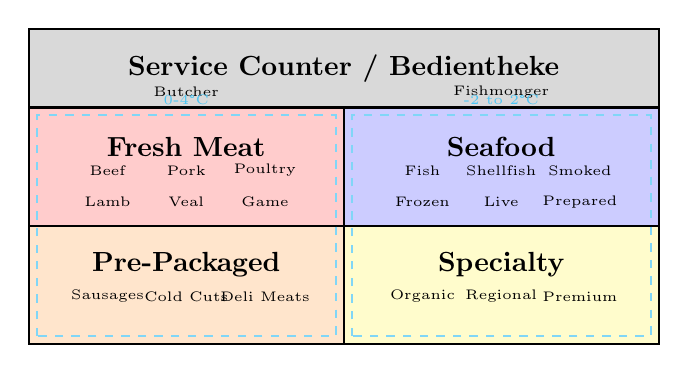
\begin{tikzpicture}[scale=1.0]
    % Section outline
    \draw[thick, fill=red!10] (0,0) rectangle (8,4);
    
    % Service counter
    \draw[thick, fill=gray!30] (0,3) rectangle (8,4);
    \node[font=\bfseries] at (4,3.5) {Service Counter / Bedientheke};
    \node[font=\tiny] at (2,3.2) {Butcher};
    \node[font=\tiny] at (6,3.2) {Fishmonger};
    
    % Meat display cases
    \draw[thick, fill=red!20] (0,1.5) rectangle (4,3);
    \node[font=\bfseries] at (2,2.5) {Fresh Meat};
    \node[font=\tiny] at (1,2.2) {Beef};
    \node[font=\tiny] at (2,2.2) {Pork};
    \node[font=\tiny] at (3,2.2) {Poultry};
    \node[font=\tiny] at (1,1.8) {Lamb};
    \node[font=\tiny] at (2,1.8) {Veal};
    \node[font=\tiny] at (3,1.8) {Game};
    
    % Seafood display cases
    \draw[thick, fill=blue!20] (4,1.5) rectangle (8,3);
    \node[font=\bfseries] at (6,2.5) {Seafood};
    \node[font=\tiny] at (5,2.2) {Fish};
    \node[font=\tiny] at (6,2.2) {Shellfish};
    \node[font=\tiny] at (7,2.2) {Smoked};
    \node[font=\tiny] at (5,1.8) {Frozen};
    \node[font=\tiny] at (6,1.8) {Live};
    \node[font=\tiny] at (7,1.8) {Prepared};
    
    % Pre-packaged section
    \draw[thick, fill=orange!20] (0,0) rectangle (4,1.5);
    \node[font=\bfseries] at (2,1) {Pre-Packaged};
    \node[font=\tiny] at (1,0.6) {Sausages};
    \node[font=\tiny] at (2,0.6) {Cold Cuts};
    \node[font=\tiny] at (3,0.6) {Deli Meats};
    
    % Specialty items
    \draw[thick, fill=yellow!20] (4,0) rectangle (8,1.5);
    \node[font=\bfseries] at (6,1) {Specialty};
    \node[font=\tiny] at (5,0.6) {Organic};
    \node[font=\tiny] at (6,0.6) {Regional};
    \node[font=\tiny] at (7,0.6) {Premium};
    
    % Temperature zones
    \draw[thick, dashed, cyan!50] (0.1,0.1) rectangle (3.9,2.9);
    \node[font=\tiny, cyan!70] at (2,3.1) {0-4°C};
    \draw[thick, dashed, cyan!50] (4.1,0.1) rectangle (7.9,2.9);
    \node[font=\tiny, cyan!70] at (6,3.1) {-2 to 2°C};
\end{tikzpicture}
\caption{Meat and Seafood Section / Fleisch- und Fischabteilung / 肉类和海鲜区}
\end{figure}

\subsection{Bakery Section / Bäckerei / 烘焙区}

\begin{otherlanguage}{ngerman}
Die Bäckerei ist oft eine der ersten Abteilungen, die Kunden sehen, da der Geruch von frischem Brot sehr anziehend wirkt. Viele Edeka-Filialen haben eine eigene Backstube.
\end{otherlanguage}

The bakery is often one of the first departments customers see, as the smell of fresh bread is very appealing. Many Edeka stores have their own baking facility.

烘焙区通常是顾客最先看到的部门之一，因为新鲜面包的香味非常吸引人。许多艾德卡门店都有自己的烘焙设施。

% Bakery Section Detail
\begin{figure}[h]
\centering
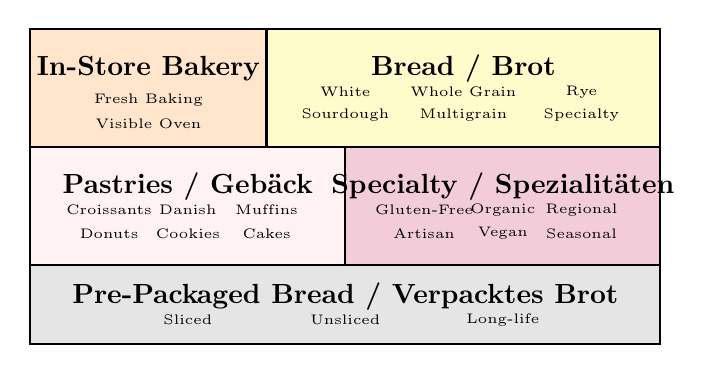
\begin{tikzpicture}[scale=1.0]
    % Section outline
    \draw[thick, fill=yellow!10] (0,0) rectangle (8,4);
    
    % In-store bakery (if present)
    \draw[thick, fill=orange!20] (0,2.5) rectangle (3,4);
    \node[font=\bfseries] at (1.5,3.5) {In-Store Bakery};
    \node[font=\tiny] at (1.5,3.1) {Fresh Baking};
    \node[font=\tiny] at (1.5,2.8) {Visible Oven};
    
    % Bread display
    \draw[thick, fill=yellow!20] (3,2.5) rectangle (8,4);
    \node[font=\bfseries] at (5.5,3.5) {Bread / Brot};
    \node[font=\tiny] at (4,3.2) {White};
    \node[font=\tiny] at (5.5,3.2) {Whole Grain};
    \node[font=\tiny] at (7,3.2) {Rye};
    \node[font=\tiny] at (4,2.9) {Sourdough};
    \node[font=\tiny] at (5.5,2.9) {Multigrain};
    \node[font=\tiny] at (7,2.9) {Specialty};
    
    % Pastries and cakes
    \draw[thick, fill=pink!20] (0,1) rectangle (4,2.5);
    \node[font=\bfseries] at (2,2) {Pastries / Gebäck};
    \node[font=\tiny] at (1,1.7) {Croissants};
    \node[font=\tiny] at (2,1.7) {Danish};
    \node[font=\tiny] at (3,1.7) {Muffins};
    \node[font=\tiny] at (1,1.4) {Donuts};
    \node[font=\tiny] at (2,1.4) {Cookies};
    \node[font=\tiny] at (3,1.4) {Cakes};
    
    % Specialty items
    \draw[thick, fill=purple!20] (4,1) rectangle (8,2.5);
    \node[font=\bfseries] at (6,2) {Specialty / Spezialitäten};
    \node[font=\tiny] at (5,1.7) {Gluten-Free};
    \node[font=\tiny] at (6,1.7) {Organic};
    \node[font=\tiny] at (7,1.7) {Regional};
    \node[font=\tiny] at (5,1.4) {Artisan};
    \node[font=\tiny] at (6,1.4) {Vegan};
    \node[font=\tiny] at (7,1.4) {Seasonal};
    
    % Pre-packaged
    \draw[thick, fill=gray!20] (0,0) rectangle (8,1);
    \node[font=\bfseries] at (4,0.6) {Pre-Packaged Bread / Verpacktes Brot};
    \node[font=\tiny] at (2,0.3) {Sliced};
    \node[font=\tiny] at (4,0.3) {Unsliced};
    \node[font=\tiny] at (6,0.3) {Long-life};
\end{tikzpicture}
\caption{Bakery Section Layout / Bäckerei-Layout / 烘焙区布局}
\end{figure}

\section{Food Services / Gastronomie / 餐饮服务}

\begin{otherlanguage}{ngerman}
Viele Edeka-Filialen bieten Food-Service-Bereiche an, die von einfachen Sitzgelegenheiten bis hin zu vollständigen Cafés oder Bistros reichen können.
\end{otherlanguage}

Many Edeka stores offer food service areas, ranging from simple seating to full cafés or bistros.

许多艾德卡门店提供餐饮服务区，从简单的座位到完整的咖啡厅或小酒馆。

% Food Service Area Detail
\begin{figure}[h]
\centering
\begin{tikzpicture}[scale=1.0]
    % Service area outline
    \draw[thick, fill=orange!10] (0,0) rectangle (10,6);
    
    % Counter/Service area
    \draw[thick, fill=gray!30] (0,4) rectangle (10,6);
    \node[font=\bfseries] at (5,5.5) {Service Counter / Theke};
    \node[font=\tiny] at (2.5,5.1) {Hot Food};
    \node[font=\tiny] at (5,5.1) {Salad Bar};
    \node[font=\tiny] at (7.5,5.1) {Beverages};
    
    % Hot food section
    \draw[thick, fill=red!20] (0,2.5) rectangle (3,4);
    \node[font=\bfseries] at (1.5,3.5) {Hot Food};
    \node[font=\tiny] at (1.5,3.2) {Soups};
    \node[font=\tiny] at (1.5,3) {Ready Meals};
    \node[font=\tiny] at (1.5,2.8) {Grill Items};
    
    % Salad bar
    \draw[thick, fill=green!20] (3,2.5) rectangle (6,4);
    \node[font=\bfseries] at (4.5,3.5) {Salad Bar};
    \node[font=\tiny] at (4.5,3.2) {Fresh Salads};
    \node[font=\tiny] at (4.5,3) {Toppings};
    \node[font=\tiny] at (4.5,2.8) {Dressings};
    
    % Beverage station
    \draw[thick, fill=blue!20] (6,2.5) rectangle (10,4);
    \node[font=\bfseries] at (8,3.5) {Beverages};
    \node[font=\tiny] at (7,3.2) {Coffee};
    \node[font=\tiny] at (8,3.2) {Tea};
    \node[font=\tiny] at (9,3.2) {Soft Drinks};
    \node[font=\tiny] at (8,3) {Juices};
    
    % Seating area
    \draw[thick, fill=beige!20] (0,0) rectangle (10,2.5);
    \node[font=\bfseries] at (5,2) {Seating Area / Sitzbereich};
    
    % Tables (represented as circles)
    \foreach \x in {1.5, 4.5, 7.5} {
        \foreach \y in {0.5, 1.5} {
            \draw[thick, fill=beige!40] (\x,\y) circle (0.3);
            \node[font=\tiny] at (\x,\y) {Table};
        }
    }
    
    % Additional services
    \draw[thick, dashed, purple!50] (0.2,0.2) rectangle (9.8,2.3);
    \node[font=\tiny, purple!70] at (5,2.4) {WiFi Available};
    \node[font=\tiny] at (2.5,0.3) {Charging};
    \node[font=\tiny] at (7.5,0.3) {Newspapers};
\end{tikzpicture}
\caption{Food Service Area Layout / Gastronomiebereich-Layout / 餐饮服务区布局}
\end{figure}

\section{Store Positioning Strategy / Filialpositionierungs-Strategie / 门店定位策略}

\begin{otherlanguage}{ngerman}
Edeka-Filialen werden strategisch positioniert, basierend auf Standorttyp, Zielgruppe und Wettbewerbssituation.
\end{otherlanguage}

Edeka stores are strategically positioned based on location type, target audience, and competitive situation.

艾德卡门店根据位置类型、目标受众和竞争情况进行战略定位。

% Store Positioning Matrix
\begin{figure}[h]
\centering
\begin{tikzpicture}[scale=1.0]
    % Axes
    \draw[->, thick] (0,0) -- (10,0) node[right] {Store Size / Filialgröße};
    \draw[->, thick] (0,0) -- (0,10) node[above, rotate=90] {Service Level / Servicelevel};
    
    % Grid
    \draw[gray!30, dashed] (0,5) -- (10,5);
    \draw[gray!30, dashed] (5,0) -- (5,10);
    
    % Store types
    \node[circle, fill=blue!70, draw=blue!90, thick, minimum size=1.5cm] (hyper) at (8.5,8.5) {};
    \node[above, font=\bfseries] at (8.5,9.5) {Hypermarket};
    \node[below, font=\tiny] at (8.5,7.5) {Large Format};
    \node[below, font=\tiny] at (8.5,7.2) {Full Service};
    
    \node[circle, fill=green!70, draw=green!90, thick, minimum size=1.2cm] (super) at (6,6.5) {};
    \node[above, font=\bfseries] at (6,7.5) {Supermarket};
    \node[below, font=\tiny] at (6,5.5) {Standard};
    \node[below, font=\tiny] at (6,5.2) {Full Range};
    
    \node[circle, fill=yellow!70, draw=yellow!90, thick, minimum size=1cm] (neighborhood) at (3,4) {};
    \node[above, font=\bfseries] at (3,5) {Neighborhood};
    \node[below, font=\tiny] at (3,3) {Compact};
    \node[below, font=\tiny] at (3,2.7) {Convenience};
    
    \node[circle, fill=orange!70, draw=orange!90, thick, minimum size=0.8cm] (express) at (1.5,2) {};
    \node[above, font=\bfseries] at (1.5,3) {Express};
    \node[below, font=\tiny] at (1.5,1) {Small};
    \node[below, font=\tiny] at (1.5,0.7) {Quick Service};
    
    % Location types
    \node[above right, font=\small, blue!70] at (0,10) {City Center};
    \node[above left, font=\small, green!70] at (10,10) {Suburban};
    \node[below right, font=\small, yellow!70] at (0,0) {Residential};
    \node[below left, font=\small, orange!70] at (10,0) {Highway};
    
    % Quadrant labels
    \node[above right, font=\tiny, gray!50] at (0,10) {Small, High Service};
    \node[above left, font=\tiny, gray!50] at (10,10) {Large, High Service};
    \node[below right, font=\tiny, gray!50] at (0,0) {Small, Low Service};
    \node[below left, font=\tiny, gray!50] at (10,0) {Large, Low Service};
    
    % Axis labels
    \node[below] at (2.5,0) {\small Small};
    \node[below] at (7.5,0) {\small Large};
    \node[left] at (0,2.5) {\small Basic};
    \node[left] at (0,7.5) {\small Full};
    
    % Title
    \node[above, font=\bfseries] at (5,10.5) {Store Positioning Strategy / Filialpositionierungs-Strategie / 门店定位策略};
\end{tikzpicture}
\caption{Store Type Positioning / Filialtyp-Positionierung / 门店类型定位}
\end{figure}

\section{Detailed Layout Equation / Detaillierte Layout-Gleichung / 详细布局公式}

\begin{otherlanguage}{ngerman}
Das Edeka-Layout folgt einer mathematischen Optimierungsgleichung, die verschiedene Faktoren berücksichtigt:
\end{otherlanguage}

The Edeka layout follows a mathematical optimization equation that considers various factors:

艾德卡布局遵循一个考虑各种因素的数学优化方程：

\begin{equation}
\text{Optimal Layout} = \max \left( \sum_{i=1}^{n} \left( R_i \times V_i \times F_i \right) - C \right)
\end{equation}

where:
\begin{itemize}
    \item $R_i$ = Revenue per square meter of section $i$
    \item $V_i$ = Customer visit frequency to section $i$
    \item $F_i$ = Flow factor (how section $i$ drives traffic to other sections)
    \item $C$ = Total operational costs
    \item $n$ = Number of sections
\end{itemize}

\begin{otherlanguage}{ngerman}
wobei:
\begin{itemize}
    \item $R_i$ = Umsatz pro Quadratmeter der Sektion $i$
    \item $V_i$ = Kundenbesuchsfrequenz in Sektion $i$
    \item $F_i$ = Flussfaktor (wie Sektion $i$ Verkehr zu anderen Sektionen lenkt)
    \item $C$ = Gesamtbetriebskosten
    \item $n$ = Anzahl der Sektionen
\end{itemize}
\end{otherlanguage}

其中：
\begin{itemize}
    \item $R_i$ = 区域$i$的每平方米收入
    \item $V_i$ = 区域$i$的客户访问频率
    \item $F_i$ = 流量因子（区域$i$如何引导流量到其他区域）
    \item $C$ = 总运营成本
    \item $n$ = 区域数量
\end{itemize}

% Detailed Section Analysis
\begin{figure}[h]
\centering
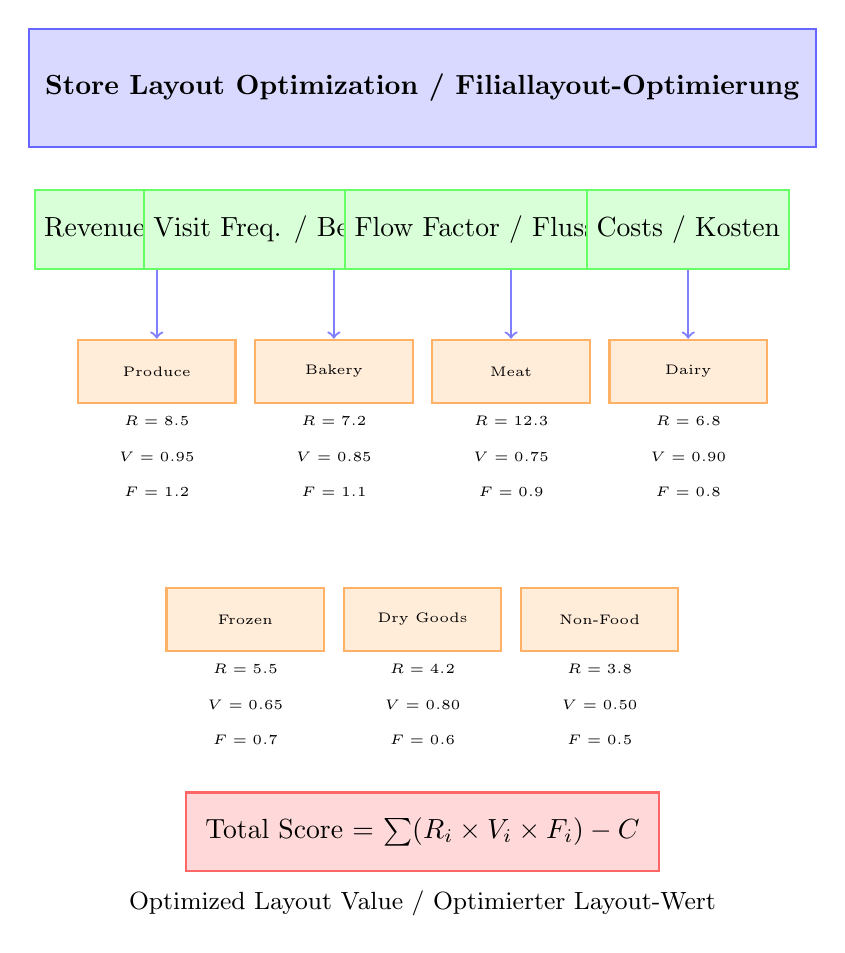
\begin{tikzpicture}[scale=0.9]
    % Create a detailed breakdown diagram
    \node[rectangle, draw=blue!60, fill=blue!15, thick, minimum width=10cm, minimum height=1.5cm, text centered] (layout) at (0,8) {\textbf{Store Layout Optimization / Filiallayout-Optimierung}};
    
    % Factors
    \node[rectangle, draw=green!60, fill=green!15, thick, minimum width=2.5cm, minimum height=1cm, text centered] (revenue) at (-3.75,6) {Revenue / Umsatz};
    \node[rectangle, draw=green!60, fill=green!15, thick, minimum width=2.5cm, minimum height=1cm, text centered] (visit) at (-1.25,6) {Visit Freq. / Besuchsfrequenz};
    \node[rectangle, draw=green!60, fill=green!15, thick, minimum width=2.5cm, minimum height=1cm, text centered] (flow) at (1.25,6) {Flow Factor / Flussfaktor};
    \node[rectangle, draw=green!60, fill=green!15, thick, minimum width=2.5cm, minimum height=1cm, text centered] (cost) at (3.75,6) {Costs / Kosten};
    
    % Sections with values
    \node[rectangle, draw=orange!60, fill=orange!15, thick, minimum width=2cm, minimum height=0.8cm, text centered, font=\tiny] (produce) at (-3.75,4) {Produce};
    \node[font=\tiny] at (-3.75,3.3) {$R=8.5$};
    \node[font=\tiny] at (-3.75,2.8) {$V=0.95$};
    \node[font=\tiny] at (-3.75,2.3) {$F=1.2$};
    
    \node[rectangle, draw=orange!60, fill=orange!15, thick, minimum width=2cm, minimum height=0.8cm, text centered, font=\tiny] (bakery) at (-1.25,4) {Bakery};
    \node[font=\tiny] at (-1.25,3.3) {$R=7.2$};
    \node[font=\tiny] at (-1.25,2.8) {$V=0.85$};
    \node[font=\tiny] at (-1.25,2.3) {$F=1.1$};
    
    \node[rectangle, draw=orange!60, fill=orange!15, thick, minimum width=2cm, minimum height=0.8cm, text centered, font=\tiny] (meat) at (1.25,4) {Meat};
    \node[font=\tiny] at (1.25,3.3) {$R=12.3$};
    \node[font=\tiny] at (1.25,2.8) {$V=0.75$};
    \node[font=\tiny] at (1.25,2.3) {$F=0.9$};
    
    \node[rectangle, draw=orange!60, fill=orange!15, thick, minimum width=2cm, minimum height=0.8cm, text centered, font=\tiny] (dairy) at (3.75,4) {Dairy};
    \node[font=\tiny] at (3.75,3.3) {$R=6.8$};
    \node[font=\tiny] at (3.75,2.8) {$V=0.90$};
    \node[font=\tiny] at (3.75,2.3) {$F=0.8$};
    
    % Additional sections
    \node[rectangle, draw=orange!60, fill=orange!15, thick, minimum width=2cm, minimum height=0.8cm, text centered, font=\tiny] (frozen) at (-2.5,0.5) {Frozen};
    \node[font=\tiny] at (-2.5,-0.2) {$R=5.5$};
    \node[font=\tiny] at (-2.5,-0.7) {$V=0.65$};
    \node[font=\tiny] at (-2.5,-1.2) {$F=0.7$};
    
    \node[rectangle, draw=orange!60, fill=orange!15, thick, minimum width=2cm, minimum height=0.8cm, text centered, font=\tiny] (dry) at (0,0.5) {Dry Goods};
    \node[font=\tiny] at (0,-0.2) {$R=4.2$};
    \node[font=\tiny] at (0,-0.7) {$V=0.80$};
    \node[font=\tiny] at (0,-1.2) {$F=0.6$};
    
    \node[rectangle, draw=orange!60, fill=orange!15, thick, minimum width=2cm, minimum height=0.8cm, text centered, font=\tiny] (nonfood) at (2.5,0.5) {Non-Food};
    \node[font=\tiny] at (2.5,-0.2) {$R=3.8$};
    \node[font=\tiny] at (2.5,-0.7) {$V=0.50$};
    \node[font=\tiny] at (2.5,-1.2) {$F=0.5$};
    
    % Connections
    \draw[->, thick, blue!50] (revenue) -- (produce);
    \draw[->, thick, blue!50] (visit) -- (bakery);
    \draw[->, thick, blue!50] (flow) -- (meat);
    \draw[->, thick, blue!50] (cost) -- (dairy);
    
    % Formula result
    \node[rectangle, draw=red!60, fill=red!15, thick, minimum width=6cm, minimum height=1cm, text centered] (result) at (0,-2.5) {Total Score = $\sum (R_i \times V_i \times F_i) - C$};
    \node[font=\small] at (0,-3.5) {Optimized Layout Value / Optimierter Layout-Wert};
\end{tikzpicture}
\caption{Layout Optimization Factors / Layout-Optimierungsfaktoren / 布局优化因素}
\end{figure}

\section{Customer Flow Patterns / Kundenflussmuster / 客户流动模式}

\begin{otherlanguage}{ngerman}
Die Analyse des Kundenflusses zeigt typische Bewegungsmuster, die bei der Layout-Gestaltung berücksichtigt werden.
\end{otherlanguage}

Customer flow analysis shows typical movement patterns that are considered in layout design.

客户流动分析显示了在布局设计中考虑的典型移动模式。

% Customer Flow Diagram
\begin{figure}[h]
\centering
\begin{tikzpicture}[scale=0.9]
    % Store outline
    \draw[thick, fill=gray!5] (0,0) rectangle (10,8);
    
    % Sections (simplified)
    \draw[thick, fill=green!20] (0.5,6) rectangle (4,8);
    \node[font=\tiny] at (2.25,7) {Produce};
    \draw[thick, fill=yellow!20] (0.5,4) rectangle (3,6);
    \node[font=\tiny] at (1.75,5) {Bakery};
    \draw[thick, fill=red!20] (3,4) rectangle (6,6);
    \node[font=\tiny] at (4.5,5) {Meat};
    \draw[thick, fill=blue!20] (6,4) rectangle (9.5,6);
    \node[font=\tiny] at (7.75,5) {Dairy};
    \draw[thick, fill=cyan!20] (0.5,2) rectangle (4,4);
    \node[font=\tiny] at (2.25,3) {Frozen};
    \draw[thick, fill=brown!20] (4,2) rectangle (9.5,4);
    \node[font=\tiny] at (6.75,3) {Dry Goods};
    \draw[thick, fill=orange!20] (0.5,0) rectangle (9.5,2);
    \node[font=\tiny] at (5,1) {Non-Food \& Checkout};
    
    % Customer flow paths (thickness indicates frequency)
    \draw[->, very thick, blue!70] (0.5,4) .. controls (2,4.5) and (2.5,5.5) .. (2.25,7);
    \draw[->, thick, blue!60] (2.25,7) .. controls (3.5,7.5) and (5,7) .. (7.75,5);
    \draw[->, thick, blue!60] (7.75,5) .. controls (8,4) and (7,3.5) .. (6.75,3);
    \draw[->, medium thick, blue!50] (6.75,3) .. controls (5,2.5) and (3,2.5) .. (2.25,3);
    \draw[->, medium thick, blue!50] (2.25,3) .. controls (1,1.5) and (3,1) .. (5,1);
    
    % Flow intensity legend
    \node[font=\tiny, above] at (10.5,7) {Flow Intensity};
    \draw[very thick, blue!70] (10,6) -- (11,6);
    \node[font=\tiny, right] at (11,6) {High (90\%+)};
    \draw[thick, blue!60] (10,5.5) -- (11,5.5);
    \node[font=\tiny, right] at (11,5.5) {Medium (60-90\%)};
    \draw[medium thick, blue!50] (10,5) -- (11,5);
    \node[font=\tiny, right] at (11,5) {Low (<60\%)};
    
    % Dwell time indicators
    \node[circle, fill=red!30, draw=red!70, thick, minimum size=0.5cm] at (2.25,7) {};
    \node[font=\tiny, red!70] at (2.25,6.5) {High Dwell};
    \node[circle, fill=yellow!30, draw=yellow!70, thick, minimum size=0.4cm] at (4.5,5) {};
    \node[font=\tiny, yellow!70] at (4.5,4.5) {Medium};
    \node[circle, fill=green!30, draw=green!70, thick, minimum size=0.3cm] at (6.75,3) {};
    \node[font=\tiny, green!70] at (6.75,2.5) {Quick};
\end{tikzpicture}
\caption{Customer Flow Patterns / Kundenflussmuster / 客户流动模式}
\end{figure}

\section{Space Allocation Analysis / Flächenzuweisungs-Analyse / 空间分配分析}

\begin{otherlanguage}{ngerman}
Die optimale Flächenzuweisung basiert auf Umsatzdichte, Gewinnmargen und strategischen Überlegungen.
\end{otherlanguage}

Optimal space allocation is based on revenue density, profit margins, and strategic considerations.

最佳空间分配基于收入密度、利润率和战略考虑。

% Space Allocation Chart
\begin{figure}[h]
\centering
\begin{tikzpicture}[scale=1.0]
    % Bar chart for space allocation
    \def\maxwidth{8}
    
    % Define sections manually with positions
    \def\sections{{"Fresh Produce", "Bakery", "Meat \\& Seafood", "Dairy \\& Refrigerated", "Frozen Foods", "Beverages", "Dry Goods", "Non-Food", "Food Service", "Checkout \\& Aisles"}}
    \def\percents{{15, 8, 12, 10, 8, 10, 15, 12, 5, 5}}
    \def\colors{{"green!70", "yellow!70", "red!70", "blue!70", "cyan!70", "purple!70", "brown!70", "pink!70", "orange!70", "gray!70"}}
    
    % Draw bars manually
    \draw[fill=green!70, draw=green!90, thick] (0,8.2) rectangle (1.2,8.8);
    \node[left, font=\tiny] at (0,8.5) {Fresh Produce};
    \node[right, font=\tiny] at (1.2,8.5) {15\%};
    
    \draw[fill=yellow!70, draw=yellow!90, thick] (0,7.4) rectangle (0.64,8.0);
    \node[left, font=\tiny] at (0,7.7) {Bakery};
    \node[right, font=\tiny] at (0.64,7.7) {8\%};
    
    \draw[fill=red!70, draw=red!90, thick] (0,6.6) rectangle (0.96,7.2);
    \node[left, font=\tiny] at (0,6.9) {Meat \& Seafood};
    \node[right, font=\tiny] at (0.96,6.9) {12\%};
    
    \draw[fill=blue!70, draw=blue!90, thick] (0,5.8) rectangle (0.8,6.4);
    \node[left, font=\tiny] at (0,6.1) {Dairy \& Refrig.};
    \node[right, font=\tiny] at (0.8,6.1) {10\%};
    
    \draw[fill=cyan!70, draw=cyan!90, thick] (0,5.0) rectangle (0.64,5.6);
    \node[left, font=\tiny] at (0,5.3) {Frozen Foods};
    \node[right, font=\tiny] at (0.64,5.3) {8\%};
    
    \draw[fill=purple!70, draw=purple!90, thick] (0,4.2) rectangle (0.8,4.8);
    \node[left, font=\tiny] at (0,4.5) {Beverages};
    \node[right, font=\tiny] at (0.8,4.5) {10\%};
    
    \draw[fill=brown!70, draw=brown!90, thick] (0,3.4) rectangle (1.2,4.0);
    \node[left, font=\tiny] at (0,3.7) {Dry Goods};
    \node[right, font=\tiny] at (1.2,3.7) {15\%};
    
    \draw[fill=pink!70, draw=pink!90, thick] (0,2.6) rectangle (0.96,3.2);
    \node[left, font=\tiny] at (0,2.9) {Non-Food};
    \node[right, font=\tiny] at (0.96,2.9) {12\%};
    
    \draw[fill=orange!70, draw=orange!90, thick] (0,1.8) rectangle (0.4,2.4);
    \node[left, font=\tiny] at (0,2.1) {Food Service};
    \node[right, font=\tiny] at (0.4,2.1) {5\%};
    
    \draw[fill=gray!70, draw=gray!90, thick] (0,1.0) rectangle (0.4,1.6);
    \node[left, font=\tiny] at (0,1.3) {Checkout \& Aisles};
    \node[right, font=\tiny] at (0.4,1.3) {5\%};
    
    % X-axis
    \draw[->, thick] (0,0.5) -- (8.5,0.5);
    \node[below] at (4.25,0.5) {Space Allocation (\%) / Flächenzuweisung (\%) / 空间分配 (\%)};
    
    % Y-axis label
    \node[rotate=90, above] at (-1.5,4.5) {Store Sections / Filialbereiche / 门店区域};
    
    % Title
    \node[above, font=\bfseries] at (4.25,9.5) {Space Allocation by Section / Flächenzuweisung nach Bereich / 各区域空间分配};
\end{tikzpicture}
\caption{Space Allocation Analysis / Flächenzuweisungs-Analyse / 空间分配分析}
\end{figure}

\section{Service Machines and Innovation Stations / Service-Automaten und Innovationsstationen / 服务机器与创新站}

\begin{otherlanguage}{ngerman}
Edeka-Filialen bieten verschiedene Service-Automaten und innovative Stationen an, die den Kundenkomfort erhöhen und zusätzliche Services bieten. Diese Maschinen sind strategisch im Eingangs- und Ausgangsbereich platziert.
\end{otherlanguage}

Edeka stores offer various service machines and innovative stations that enhance customer convenience and provide additional services. These machines are strategically placed in the entrance and exit areas.

艾德卡门店提供各种服务机器和创新站，提高客户便利性并提供额外服务。这些机器战略性地放置在入口和出口区域。

\subsection{Existing Service Machines / Bestehende Service-Automaten / 现有服务机器}

\begin{otherlanguage}{ngerman}
\subsubsection{Leergut-Rückgabeautomaten (Pfand) / Bottle Return Machines}
Leergut-Rückgabeautomaten ermöglichen es Kunden, Pfandflaschen und -dosen zurückzugeben und erhalten sofort einen Bon, der an der Kasse eingelöst werden kann. Dies ist ein wichtiger Service in Deutschland, wo das Pfandsystem weit verbreitet ist.
\end{otherlanguage}

\subsubsection{Leergut-Rückgabeautomaten (Pfand) / Bottle Return Machines}
Bottle return machines allow customers to return deposit bottles and cans and immediately receive a voucher that can be redeemed at checkout. This is an important service in Germany, where the deposit system is widespread.

\subsubsection{Leergut-Rückgabeautomaten (Pfand) / 瓶子回收机}
瓶子回收机允许顾客退回押金瓶和罐子，并立即获得可在收银台兑换的凭证。这是德国的一项重要服务，押金系统在那里很普遍。

\begin{otherlanguage}{ngerman}
\subsubsection{Coinstar-Münzzählmaschinen}
Coinstar-Maschinen zählen Münzen und geben einen Wertbon aus, der im Geschäft eingelöst werden kann. Dies ist besonders nützlich für Kunden, die große Mengen an Kleingeld haben.
\end{otherlanguage}

\subsubsection{Coinstar Coin Counting Machines}
Coinstar machines count coins and issue a value voucher that can be redeemed in the store. This is particularly useful for customers who have large amounts of loose change.

\subsubsection{Coinstar硬币计数机}
Coinstar机器计算硬币并发放可在店内兑换的价值券。这对拥有大量零钱的顾客特别有用。

% Service Machines Layout
\begin{figure}[h]
\centering
\begin{tikzpicture}[scale=1.0]
    % Store entrance area
    \draw[thick, fill=gray!10] (0,0) rectangle (10,6);
    
    % Entrance
    \draw[thick, fill=green!30] (0,2) rectangle (1,4);
    \node[rotate=90, font=\small\bfseries] at (0.5,3) {ENTRANCE};
    
    % Service machines area
    \draw[thick, fill=blue!15, dashed] (1,0.5) rectangle (9,5.5);
    \node[font=\bfseries, above] at (5,5.5) {Service Machines Area / Service-Automaten-Bereich / 服务机器区};
    
    % Leergut machine
    \draw[thick, fill=green!30] (1.5,3.5) rectangle (3,5);
    \node[font=\tiny\bfseries, text width=1.3cm, text centered] at (2.25,4.5) {Leergut};
    \node[font=\tiny\bfseries, text width=1.3cm, text centered] at (2.25,4.2) {Pfand};
    \node[font=\tiny, text width=1.3cm, text centered] at (2.25,3.8) {Bottle Return};
    \draw[thick, fill=green!50] (2.25,3.5) circle (0.15);
    \node[font=\tiny] at (2.25,3.2) {Deposit};
    
    % Coinstar machine
    \draw[thick, fill=yellow!30] (3.5,3.5) rectangle (5,5);
    \node[font=\tiny\bfseries, text width=1.3cm, text centered] at (4.25,4.5) {Coinstar};
    \node[font=\tiny, text width=1.3cm, text centered] at (4.25,4.2) {Coin};
    \node[font=\tiny, text width=1.3cm, text centered] at (4.25,3.8) {Counter};
    \draw[thick, fill=yellow!50] (4.25,3.5) circle (0.15);
    \node[font=\tiny] at (4.25,3.2) {Wertbon};
    
    % Innovative machines (to be added)
    \draw[thick, fill=purple!30] (5.5,3.5) rectangle (7,5);
    \node[font=\tiny\bfseries, text width=1.3cm, text centered] at (6.25,4.5) {Smart};
    \node[font=\tiny\bfseries, text width=1.3cm, text centered] at (6.25,4.2) {Locker};
    \node[font=\tiny, text width=1.3cm, text centered] at (6.25,3.8) {Pickup};
    \draw[thick, fill=purple!50] (6.25,3.5) circle (0.15);
    \node[font=\tiny] at (6.25,3.2) {Online Orders};
    
    \draw[thick, fill=orange!30] (7.5,3.5) rectangle (9,5);
    \node[font=\tiny\bfseries, text width=1.3cm, text centered] at (8.25,4.5) {Digital};
    \node[font=\tiny\bfseries, text width=1.3cm, text centered] at (8.25,4.2) {Kiosk};
    \node[font=\tiny, text width=1.3cm, text centered] at (8.25,3.8) {Services};
    \draw[thick, fill=orange!50] (8.25,3.5) circle (0.15);
    \node[font=\tiny] at (8.25,3.2) {Multi-Service};
    
    % Charging stations
    \draw[thick, fill=cyan!20] (1.5,1.5) rectangle (3,3);
    \node[font=\tiny\bfseries, text width=1.3cm, text centered] at (2.25,2.5) {Mobile};
    \node[font=\tiny\bfseries, text width=1.3cm, text centered] at (2.25,2.2) {Charging};
    \node[font=\tiny, text width=1.3cm, text centered] at (2.25,1.8) {Station};
    \draw[thick, fill=cyan!40] (2.25,1.5) circle (0.1);
    \node[font=\tiny] at (2.25,1.3) {USB/Wireless};
    
    % Recycling station
    \draw[thick, fill=green!20] (3.5,1.5) rectangle (5,3);
    \node[font=\tiny\bfseries, text width=1.3cm, text centered] at (4.25,2.5) {Smart};
    \node[font=\tiny\bfseries, text width=1.3cm, text centered] at (4.25,2.2) {Recycling};
    \node[font=\tiny, text width=1.3cm, text centered] at (4.25,1.8) {Station};
    \draw[thick, fill=green!40] (4.25,1.5) circle (0.1);
    \node[font=\tiny] at (4.25,1.3) {Rewards};
    
    % Price checker
    \draw[thick, fill=red!20] (5.5,1.5) rectangle (7,3);
    \node[font=\tiny\bfseries, text width=1.3cm, text centered] at (6.25,2.5) {Digital};
    \node[font=\tiny\bfseries, text width=1.3cm, text centered] at (6.25,2.2) {Price};
    \node[font=\tiny, text width=1.3cm, text centered] at (6.25,1.8) {Checker};
    \draw[thick, fill=red!40] (6.25,1.5) circle (0.1);
    \node[font=\tiny] at (6.25,1.3) {QR/Scan};
    
    % Gift card machine
    \draw[thick, fill=pink!20] (7.5,1.5) rectangle (9,3);
    \node[font=\tiny\bfseries, text width=1.3cm, text centered] at (8.25,2.5) {Gift Card};
    \node[font=\tiny\bfseries, text width=1.3cm, text centered] at (8.25,2.2) {Machine};
    \node[font=\tiny, text width=1.3cm, text centered] at (8.25,1.8) {Instant};
    \draw[thick, fill=pink!40] (8.25,1.5) circle (0.1);
    \node[font=\tiny] at (8.25,1.3) {Print};
    
    % Arrows showing flow
    \draw[->, thick, blue!50] (1,3) -- (1.5,3);
    \draw[->, thick, blue!50] (3,4.25) -- (3.5,4.25);
    \draw[->, thick, blue!50] (5,4.25) -- (5.5,4.25);
    \draw[->, thick, blue!50] (7,4.25) -- (7.5,4.25);
    
    % Checkout direction
    \draw[->, thick, red!50] (9,3) -- (10,3);
    \node[right, font=\tiny] at (10,3) {To Checkout};
\end{tikzpicture}
\caption{Service Machines Layout / Service-Automaten-Layout / 服务机器布局}
\end{figure}

\subsection{Innovative Service Ideas / Innovative Service-Ideen / 创新服务理念}

\begin{otherlanguage}{ngerman}
Neben den bestehenden Maschinen gibt es zahlreiche innovative Ideen, die Edeka implementieren könnte, um die Kundenerfahrung zu verbessern und zusätzliche Services anzubieten.
\end{otherlanguage}

Beyond existing machines, there are numerous innovative ideas that Edeka could implement to enhance customer experience and offer additional services.

除了现有机器外，还有许多创新理念，艾德卡可以实施这些理念来增强客户体验并提供额外服务。

\subsubsection{Smart Package Lockers / Intelligente Paketstationen / 智能包裹柜}

\begin{otherlanguage}{ngerman}
Intelligente Paketstationen ermöglichen es Kunden, Online-Bestellungen abzuholen, ohne in die Schlange zu gehen. Diese können auch für Click \& Collect-Bestellungen verwendet werden.
\end{otherlanguage}

Smart package lockers allow customers to pick up online orders without queuing. These can also be used for click \& collect orders.

智能包裹柜允许顾客无需排队即可取走在线订单。这些也可用于点击取货订单。

\textbf{Features / Funktionen / 功能}:
\begin{itemize}
    \item QR-Code-Scanner für schnelle Abholung / QR code scanner for quick pickup / 二维码扫描快速取货
    \item Temperaturkontrollierte Fächer für frische Produkte / Temperature-controlled compartments for fresh products / 新鲜产品的温控隔间
    \item 24/7-Verfügbarkeit / 24/7 availability / 24/7可用性
    \item SMS/E-Mail-Benachrichtigungen / SMS/email notifications / 短信/电子邮件通知
\end{itemize}

\subsubsection{Digital Service Kiosk / Digitaler Service-Kiosk / 数字服务亭}

\begin{otherlanguage}{ngerman}
Ein multifunktionaler digitaler Kiosk, der verschiedene Services anbietet:
\end{otherlanguage}

A multifunctional digital kiosk offering various services:

提供各种服务的多功能数字亭：

\textbf{Services / Dienstleistungen / 服务}:
\begin{itemize}
    \item Produktinformationen und Verfügbarkeit / Product information and availability / 产品信息和可用性
    \item Rezeptvorschläge basierend auf gekauften Produkten / Recipe suggestions based on purchased products / 根据购买的产品提供食谱建议
    \item Treueprogramm-Verwaltung / Loyalty program management / 忠诚度计划管理
    \item Geschenkkarten-Kauf und -Aufladung / Gift card purchase and reload / 礼品卡购买和充值
    \item Rückgabe- und Umtausch-Service / Return and exchange service / 退货和换货服务
    \item Lokale Veranstaltungen und Angebote / Local events and offers / 本地活动和优惠
\end{itemize}

\subsubsection{Mobile Charging Stations / Mobile Ladestationen / 移动充电站}

\begin{otherlanguage}{ngerman}
Strategisch platzierte Ladestationen für Smartphones und andere Geräte, die Kunden während des Einkaufs nutzen können.
\end{otherlanguage}

Strategically placed charging stations for smartphones and other devices that customers can use while shopping.

战略性放置的智能手机和其他设备充电站，顾客在购物时可以使用。

\textbf{Features / Funktionen / 功能}:
\begin{itemize}
    \item USB-C, USB-A und drahtlose Ladung / USB-C, USB-A, and wireless charging / USB-C、USB-A和无线充电
    \item Sicherheitsfächer für Geräte / Secure lockers for devices / 设备安全柜
    \item Schnellladefunktion / Fast charging capability / 快速充电功能
    \item Integration mit Edeka-App für Benachrichtigungen / Integration with Edeka app for notifications / 与艾德卡应用集成以接收通知
\end{itemize}

\subsubsection{Smart Recycling Station / Intelligente Recycling-Station / 智能回收站}

\begin{otherlanguage}{ngerman}
Eine erweiterte Recycling-Station, die nicht nur Pfandflaschen, sondern auch andere Materialien akzeptiert und Belohnungen bietet.
\end{otherlanguage}

An advanced recycling station that accepts not only deposit bottles but also other materials and offers rewards.

一个先进的回收站，不仅接受押金瓶，还接受其他材料并提供奖励。

\textbf{Features / Funktionen / 功能}:
\begin{itemize}
    \item Elektronik-Recycling (alte Handys, Tablets) / Electronics recycling (old phones, tablets) / 电子产品回收（旧手机、平板电脑）
    \item Batterie-Recycling / Battery recycling / 电池回收
    \item Plastikverpackungen / Plastic packaging / 塑料包装
    \item Belohnungspunkte für Recycling / Reward points for recycling / 回收奖励积分
    \item CO2-Fußabdruck-Tracking / CO2 footprint tracking / 二氧化碳足迹跟踪
\end{itemize}

\subsubsection{Digital Price Checker / Digitaler Preisprüfer / 数字价格检查器}

\begin{otherlanguage}{ngerman}
Interaktive Displays, die Kunden ermöglichen, Preise zu überprüfen, Produktinformationen abzurufen und Alternativen zu finden.
\end{otherlanguage}

Interactive displays that allow customers to check prices, retrieve product information, and find alternatives.

允许顾客检查价格、检索产品信息并查找替代品的交互式显示屏。

\textbf{Features / Funktionen / 功能}:
\begin{itemize}
    \item Barcode-Scanner / Barcode scanner / 条形码扫描器
    \item QR-Code-Scanner / QR code scanner / 二维码扫描器
    \item Produktvergleich / Product comparison / 产品比较
    \item Allergen-Informationen / Allergen information / 过敏原信息
    \item Nährwertangaben / Nutritional information / 营养信息
    \item Verfügbarkeit in anderen Filialen / Availability in other stores / 其他门店的可用性
\end{itemize}

\subsubsection{Instant Gift Card Machine / Sofort-Geschenkkarten-Automat / 即时礼品卡机}

\begin{otherlanguage}{ngerman}
Ein Automat, der sofort personalisierte Geschenkkarten druckt und aktiviert.
\end{otherlanguage}

A machine that instantly prints and activates personalized gift cards.

即时打印并激活个性化礼品卡的机器。

\textbf{Features / Funktionen / 功能}:
\begin{itemize}
    \item Wählbare Beträge / Selectable amounts / 可选金额
    \item Personalisierte Designs / Personalized designs / 个性化设计
    \item Sofortige Aktivierung / Instant activation / 即时激活
    \item Digital oder physisch / Digital or physical / 数字或实体
    \item Versandoptionen / Shipping options / 配送选项
\end{itemize}

\subsubsection{AI-Powered Shopping Assistant / KI-gestützter Einkaufsassistent / AI驱动的购物助手}

\begin{otherlanguage}{ngerman}
Ein intelligenter Einkaufsassistent, der Kunden durch den Laden führt und personalisierte Empfehlungen gibt.
\end{otherlanguage}

An intelligent shopping assistant that guides customers through the store and provides personalized recommendations.

智能购物助手，引导顾客在店内购物并提供个性化推荐。

\textbf{Features / Funktionen / 功能}:
\begin{itemize}
    \item Sprachsteuerung / Voice control / 语音控制
    \item Personalisierte Einkaufslisten / Personalized shopping lists / 个性化购物清单
    \item Rezeptvorschläge basierend auf Vorlieben / Recipe suggestions based on preferences / 根据偏好提供食谱建议
    \item Navigation zu Produkten / Navigation to products / 产品导航
    \item Preisalarme und Angebote / Price alerts and offers / 价格提醒和优惠
    \item Integration mit Smart Home / Integration with smart home / 与智能家居集成
\end{itemize}

\subsubsection{Food Waste Reduction Station / Lebensmittelverschwendungs-Reduktionsstation / 食物浪费减少站}

\begin{otherlanguage}{ngerman}
Eine Station, die kurz vor dem Ablaufdatum stehende Produkte zu reduzierten Preisen anbietet und Kunden über nachhaltige Einkaufsgewohnheiten informiert.
\end{otherlanguage}

A station offering products near expiration at reduced prices and educating customers about sustainable shopping habits.

以折扣价提供即将过期的产品并教育顾客可持续购物习惯的站点。

\textbf{Features / Funktionen / 功能}:
\begin{itemize}
    \item Automatische Preisreduzierung / Automatic price reduction / 自动降价
    \item Bildungsinformationen / Educational information / 教育信息
    \item Rezepte für "Resteverwertung" / Recipes for "leftover utilization" / "剩菜利用"食谱
    \item Spendenoption für lokale Tafeln / Donation option for local food banks / 向当地食品银行捐赠的选项
    \item Tracking des eingesparten CO2 / Tracking of saved CO2 / 跟踪节省的二氧化碳
\end{itemize}

% Innovation Impact Diagram
\begin{figure}[h]
\centering
\begin{tikzpicture}[scale=1.0]
    % Central hub
    \node[circle, draw=blue!70, fill=blue!20, thick, minimum size=2cm, text centered] (hub) at (5,5) {\textbf{Customer} \\ \textbf{Experience}};
    
    % Innovation categories
    \node[rectangle, draw=green!70, fill=green!20, thick, minimum width=2.5cm, minimum height=1cm, text centered] (convenience) at (1,7) {Convenience / Bequemlichkeit};
    \node[rectangle, draw=orange!70, fill=orange!20, thick, minimum width=2.5cm, minimum height=1cm, text centered] (sustainability) at (9,7) {Sustainability / Nachhaltigkeit};
    \node[rectangle, draw=purple!70, fill=purple!20, thick, minimum width=2.5cm, minimum height=1cm, text centered] (technology) at (1,3) {Technology / Technologie};
    \node[rectangle, draw=red!70, fill=red!20, thick, minimum width=2.5cm, minimum height=1cm, text centered] (engagement) at (9,3) {Engagement / Engagement};
    
    % Specific innovations
    \node[ellipse, draw=green!50, fill=green!10, thick, minimum width=1.8cm, minimum height=0.6cm, text centered, font=\tiny, shape=ellipse] (locker) at (0.5,8.5) {Smart Lockers};
    \node[ellipse, draw=green!50, fill=green!10, thick, minimum width=1.8cm, minimum height=0.6cm, text centered, font=\tiny, shape=ellipse] (charging) at (1.5,5.5) {Charging};
    \node[ellipse, draw=orange!50, fill=orange!10, thick, minimum width=1.8cm, minimum height=0.6cm, text centered, font=\tiny, shape=ellipse] (recycle) at (9.5,8.5) {Recycling};
    \node[ellipse, draw=orange!50, fill=orange!10, thick, minimum width=1.8cm, minimum height=0.6cm, text centered, font=\tiny, shape=ellipse] (waste) at (8.5,5.5) {Waste Reduction};
    \node[ellipse, draw=purple!50, fill=purple!10, thick, minimum width=1.8cm, minimum height=0.6cm, text centered, font=\tiny, shape=ellipse] (kiosk) at (0.5,1.5) {Digital Kiosk};
    \node[ellipse, draw=purple!50, fill=purple!10, thick, minimum width=1.8cm, minimum height=0.6cm, text centered, font=\tiny, shape=ellipse] (ai) at (1.5,2.5) {AI Assistant};
    \node[ellipse, draw=red!50, fill=red!10, thick, minimum width=1.8cm, minimum height=0.6cm, text centered, font=\tiny, shape=ellipse] (price) at (9.5,1.5) {Price Checker};
    \node[ellipse, draw=red!50, fill=red!10, thick, minimum width=1.8cm, minimum height=0.6cm, text centered, font=\tiny, shape=ellipse] (gift) at (8.5,2.5) {Gift Cards};
    
    % Connections
    \draw[->, thick, green!50] (convenience) -- (hub);
    \draw[->, thick, orange!50] (sustainability) -- (hub);
    \draw[->, thick, purple!50] (technology) -- (hub);
    \draw[->, thick, red!50] (engagement) -- (hub);
    
    \draw[->, thin, green!40] (locker) -- (convenience);
    \draw[->, thin, green!40] (charging) -- (convenience);
    \draw[->, thin, orange!40] (recycle) -- (sustainability);
    \draw[->, thin, orange!40] (waste) -- (sustainability);
    \draw[->, thin, purple!40] (kiosk) -- (technology);
    \draw[->, thin, purple!40] (ai) -- (technology);
    \draw[->, thin, red!40] (price) -- (engagement);
    \draw[->, thin, red!40] (gift) -- (engagement);
    
    % Title
    \node[above, font=\bfseries] at (5,9.5) {Innovation Impact Framework / Innovations-Wirkungsrahmen / 创新影响框架};
\end{tikzpicture}
\caption{Innovation Categories and Impact / Innovationskategorien und Wirkung / 创新类别与影响}
\end{figure}

\section{Conclusion / Fazit / 结论}

\begin{otherlanguage}{ngerman}
Das Edeka-Supermarkt-Layout ist das Ergebnis einer sorgfältigen Optimierung verschiedener Faktoren, die darauf abzielen, den Kundenfluss zu maximieren, den Umsatz zu steigern und gleichzeitig eine angenehme Einkaufserfahrung zu bieten. Die Integration innovativer Service-Automaten und Technologien erweitert das Serviceangebot und verbessert die Gesamterfahrung der Kunden erheblich.
\end{otherlanguage}

The Edeka supermarket layout is the result of careful optimization of various factors aimed at maximizing customer flow, increasing revenue, while providing a pleasant shopping experience. The integration of innovative service machines and technologies expands the service offering and significantly improves the overall customer experience.

艾德卡超市布局是仔细优化各种因素的结果，旨在最大化客户流量、增加收入，同时提供愉快的购物体验。创新服务机器和技术的集成扩展了服务范围，并显著改善了整体客户体验。
